\documentclass{article}
\usepackage[preprint]{neurips}
\usepackage[utf8]{inputenc}
\usepackage[T1]{fontenc}
\usepackage{hyperref}
\usepackage{url}
\usepackage{booktabs}
\usepackage{amsfonts,amsmath,amssymb}
\usepackage{microtype}
\usepackage{graphicx}
\usepackage{xcolor}
\usepackage{tcolorbox}
\graphicspath{{../figures/}}

\title{Calibrated Is Not Actionable:\\
Physics-Guided Posterior Distillation for Methane Source Attribution}

\author{Anonymous Author(s)\\ Affiliation\\ \texttt{email}}

\begin{document}
\maketitle

\begin{abstract}
The physics allows 7 meters; regulators ask for 50; a calibrated neural
localizer delivers 94. On a methane-configured testbed (500\,m site, Gaussian
plume under realistic meandering wind, 4--12 fixed masts) where the
\emph{exact} Bayesian posterior of every scenario is computable, a
conformal-wrapped deep localizer attains verified $90\%$ coverage while its
median search region has a 94\,m equivalent radius --- honestly calibrated,
nearly twice the U.S.~EPA super-emitter actionability radius, and an order of
magnitude above the 7\,m information limit. We diagnose this gap by running the
\emph{same conformal audit on every stage of the pipeline}: the sensors support
7\,m; the tempered exact-posterior teacher used for distillation supports
11.7\,m; the trained student delivers 74\,m --- and neither sharper targets
(87\,m) nor a spatially aware transport loss (243\,m) help. The bottleneck is a
computation, not supervision: set encoders cannot perform per-cell matched
filtering internally. We therefore hand the network the classical
matched-filter statistics of the known forward model as input maps, through a
zero-initialized residual head, while distilling the tempered exact posterior
--- a drop-in recipe for any localizer. Across three architecture families
(DeepSets, GNN, Set Transformer) and three seeds each, the recipe brings every
model under the 50\,m bar (44--49\,m; coverage $0.89$--$0.91$; sharper on
$91$--$96\%$ of scenarios, paired $p<10^{-200}$), while collapsing the
spread between architectures. Calibration alone does not make ML monitoring
actionable; auditing against the physics limit, and giving the network the
physics it cannot rediscover, can.
\end{abstract}

\section{Introduction}

Methane is the highest-leverage near-term climate lever: roughly $80\times$ the
20-year warming potency of CO$_2$, a $\sim$decade atmospheric lifetime, and a
heavy concentration of emissions in a small number of fixable oil-and-gas
super-emitters. Detection is increasingly solved --- UNEP's Methane Alert and
Response System issued over a thousand satellite notifications in its first two
years --- but only $\sim\!1\%$ led to documented action [UNEP, 2024]. The
missing step is \emph{attribution}: converting a detection into a source
location precise enough, and trustworthy enough, to dispatch a crew or attach a
reporting obligation. The U.S.~EPA Super-Emitter Program operationalizes
``precise enough'' as a 50\,m radius [U.S. EPA, 2024]; the EU methane
regulation and OGMP~2.0 impose analogous source-level accounting duties
[European Union, 2024]. We treat 50\,m as a concrete engineering target.

Continuous monitoring with sparse networks of fixed point sensors is the tier
of the monitoring stack where attribution must happen: a handful of cheap masts
around a facility, always on, catching the plume as it sweeps across them under
naturally meandering wind. A learned localizer can map readings to a heatmap of
candidate sources, and split conformal prediction [Angelopoulos \& Bates, 2023]
can convert the heatmap into a region guaranteed to contain the true source
$90\%$ of the time. Coverage, however, is a statement about frequency, not
usefulness: a region can be honestly $90\%$ and still be far too large to act
on. This paper is about measuring that gap exactly, diagnosing its mechanism,
and closing it.

\textbf{Contributions.} (1)~An \emph{exact-posterior audit}: a testbed whose
closed-form physics makes the true Bayesian posterior of every scenario
computable, so the efficiency of any calibrated localizer can be measured
against the information limit, in meters, against the regulatory radius.
(2)~A \emph{diagnosis by elimination}, including a new one-run diagnostic ---
conformalizing the \emph{teacher} of a distillation setup --- that decomposes
the calibrated-sharpness gap into a supervision ceiling versus a student
approximation failure. (3)~\emph{Physics-guided posterior distillation}: a
drop-in recipe (matched-filter input maps + zero-initialized residual head +
tempered exact-posterior distillation) that brings three different localizer
architectures under the 50\,m actionability radius with the coverage guarantee
intact. We claim no new conformal algorithm, no new architecture, no coverage
under distribution shift, and no field deployment.

\begin{figure}[t]
\centering
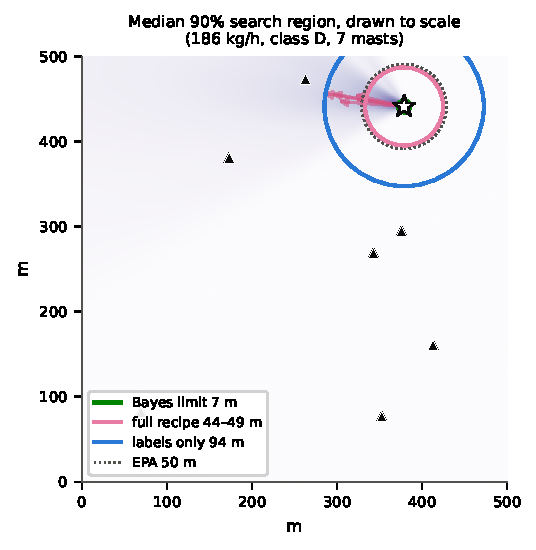
\includegraphics[width=0.58\linewidth]{figT2_example.pdf}
\caption{\textbf{The problem, to scale.} A wind-swept methane plume (purple;
meander arrows), 7 masts (black), and the true source (star) on a 500\,m site.
Circles: the median $90\%$ search region the data supports (Bayes limit, 7\,m),
what a standard calibrated localizer delivers (94\,m), and the EPA 50\,m
actionability radius sits between them. Calibration is not actionability.}
\label{fig:circles}
\end{figure}

\section{Testbed: exact posteriors as an instrument}

CH4-T places a source of unknown location and rate ($10$--$500$\,kg/h,
log-uniform) on a $500\times500$\,m site sensed by $4$--$12$ masts (ppm
readings, $0.2$--$3$\,ppm noise, dropout). The plume is a steady 3-D Gaussian
under Pasquill--Gifford stability (known class, Briggs open-country
dispersion), driven quasi-statically by a \emph{known, fluctuating} wind record
(mean $1$--$8$\,m/s with AR(1) meander in direction and speed) --- the wind
that on-site anemometry measures. As the wind veers, the plume sweeps the
masts; time-of-arrival information localizes sources that a constant wind
cannot (weakly identifiable scenarios drop from $57\%$ to $6\%$).

Because the response is closed-form and linear in the rate, the \emph{exact}
posterior over a $64\times64$ grid (cell-level attribution; sources on the
grid) is computable per scenario: a Gaussian likelihood whose rate
marginalization is done by an adaptive quadrature, validated by a blocking
self-calibration gate --- conformal prediction applied to the exact posterior
itself must recover nominal coverage (it does: $0.95$), a gate that caught a
real forward-model bug during development. The exact posterior serves twice:
as the \emph{reference} that turns ``how sharp could a calibrated region be''
into a number, and as a \emph{teacher}. All models below use identical data
($10$k/$1$k/$2$k/$2$k train/val/calib/test), identical D4 symmetry
augmentation (without which set encoders memorize), and an identical
randomized-HPD split-conformal wrapper at verified $90\%$ coverage, computed
in numerically safe tail-mass form, in float64. Region sizes are reported as
the radius of the circle of equal area; the domain is 25\,ha.

\section{Diagnosis: interrogate every stage with the same instrument}
\label{sec:diagnosis}

\textbf{Calibrated $\neq$ actionable.} A DeepSets localizer trained on
smoothed one-hot labels (M0) is well calibrated under conformal ($0.89$) yet
its median region radius is $94$\,m --- $13\times$ the Bayes limit in radius,
$\sim\!180\times$ in area. The information was in the readings; the model
could not extract it.

\textbf{The teacher is not the bottleneck.} Distilling the exact posterior ---
same network, same data, only the target changes --- requires tempering: the
raw near-delta posterior fails outright ($134$\,m, \emph{worse than no
physics}), while a $0.75$-cell Gaussian blur of it works ($74$\,m). It is
tempting to blame the blur for the remaining gap. Our diagnostic says
otherwise: run the conformal audit \emph{on the tempered teacher itself}. The
teacher supports $11.7$\,m. A perfect student of the existing lesson would
already be $6\times$ sharper than the actual student; the binding constraint
is the student's failure to match its teacher, not the lesson.

\textbf{Supervision cannot fix it.} Two controlled attempts to repair training
--- annealing the temper toward the raw posterior ($0.75\!\to\!0.15$ cells:
$87$\,m, worse), and replacing cross-entropy with a debiased Sinkhorn
(optimal-transport) divergence to the raw posterior with coarse-to-fine
$\varepsilon$-scaling ($243$\,m) --- both fail while remaining calibrated. (We
scope the transport result to our implementation; it does not preclude better
OT variants.)

\textbf{Verdict: a computation deficit.} The evidence indicates the encoder
cannot represent the required computation: identifying the source demands
correlating each of $4{,}096$ candidate cells' predicted space--time signature
against all readings --- per-cell matched filtering --- which a pooled set
representation cannot carry. No target and no loss teaches a network what its
forward pass cannot compute.

\section{Method: physics-guided posterior distillation}

The forward model is known; the computation the network lacks has a formula.
The recipe hands it over and lets learning do the rest. For any base
localizer:

\textbf{(1) Physics maps.} From the observed readings $y$, wind record, and
stability class, compute per cell $c$ the sufficient statistics of the
linear-Gaussian model, $a_c=\sum g_c y$ and $b_c=\sum g_c^2$ (with $g_c$ the
unit-rate response), and feed two $64\times64$ channels: the matched-filter
statistic $z_c=a_c/(\sigma\sqrt{b_c})$ --- classical detection theory --- and
a sensitivity map $\log b_c$. Milliseconds, closed-form, computed from the
same inputs the network already receives (no extra information; a
computation).

\textbf{(2) Zero-initialized residual head.} A 3-layer conv head reads the
maps and adds to the base model's logits. Zero-initialized final layer: at
step~0 the model \emph{is} the baseline; training opens the physics channel
only where it reduces loss. The recipe is drop-in for any architecture and
the comparison is controlled by construction.

\textbf{(3) Tempered posterior distillation.} Cross-entropy to the
$0.75$-cell-blurred exact posterior. The maps supply evidence; the teacher
teaches how to weigh evidence into a calibrated probability shape (rate
prior, noise level, multi-modality). \textbf{(4)} The unchanged conformal
wrapper certifies the result.

\begin{tcolorbox}[title=Why not just use the teacher?,left=1mm,right=1mm,top=0.5mm,bottom=0.5mm]
\small On this testbed one should --- the exact posterior is our measuring
instrument, computable by construction. In deployment it vanishes: realistic
dispersion (terrain, transients) has no closed form, and simulator inversion
costs hours per event [Newman et al., 2024] where monitoring needs seconds
across thousands of sites. Amortization is the accepted answer; what was
missing is what it \emph{costs}. And ``the teacher is just part of the
dataset'' is our thesis, not an objection: every simulated training set
already contains its own uncertainty labels; standard training throws them
away. The recipe is how to get them back --- and what must be handed over
(a matched filter) before they become learnable.
\end{tcolorbox}

\section{Results: one recipe, three architectures, all under the bar}

\begin{table}[h]
\centering\small
\caption{Median $90\%$ conformal region radius (m) on 2{,}000 test scenarios;
range over 3 seeds. Every cell is calibrated (coverage $0.887$--$0.910$).
References: Bayes limit $7.0$\,m, tempered-teacher ceiling $11.7$\,m,
\textbf{EPA actionability $50$\,m}. Baseline columns for GNN/Set Transformer
reproduce companion architecture work on the identical harness.}
\begin{tabular}{lccc}
\toprule
Architecture & Labels only & + Distillation & + \textbf{Full recipe} \\
\midrule
DeepSets (4.9M)        & 94--98 & 73--74 & \textbf{48.1--49.3} \\
GNN (5.6M)             & 55--58 & 49--52 & \textbf{43.6--44.3} \\
Set Transformer (6.5M) & 69--75 & 56--60 & \textbf{44.7--48.9} \\
\bottomrule
\end{tabular}
\label{tab:factorial}
\end{table}

Three observations. \textbf{(i)~Universality:} nine of nine seed-runs of the
recipe land under the 50\,m radius; each improves its architecture's distilled
baseline on $91$--$96\%$ of scenarios (paired Wilcoxon on log region size,
$p<10^{-200}$). \textbf{(ii)~Not a crutch for weak encoders:} the best
architecture (GNN, whose relational structure already computes pairwise
mast--wind geometry) also improves, from $49$--$52$ to $43.6$--$44.3$\,m.
\textbf{(iii)~Architecture stops mattering:} the labels-only spread across
architectures ($94$ vs.\ $56$\,m) collapses under the recipe ($49$ vs.\
$44$\,m) --- supervision and inputs, not encoder design, were the binding
constraint. Point accuracy is essentially unchanged throughout; what the
recipe changes is the \emph{shape of uncertainty}, which is what the region
size measures. Inference cost is unchanged ($\sim$ms; the maps add
milliseconds of closed-form computation).

\section{Limitations and outlook}

CH4-T is an instrument, not a deployment: steady release, flat terrain, known
stability class, quasi-static plume sensed in 2-D, \emph{exactly known} wind,
marginal in-distribution coverage. The residual factor of $\sim\!6$ between
the recipe ($44$--$49$\,m) and the Bayes limit ($7$\,m) is unexplained
headroom. The sufficiency of the input maps is exact only under the testbed's
linear-Gaussian forward model; under misspecification they are informative
features, not sufficient statistics. We have not compared against continuous
density estimators (normalizing-flow posterior estimation), and our transport
-loss null is implementation-scoped. Measured-wind uncertainty --- anemometer
error, the deployment reality --- is the immediate next act: the Bayes-correct
response (wind-marginalized teachers and ensemble physics maps) is implemented
and under evaluation. The path to field claims runs through controlled-release
data (METEC-style); what this study establishes is the reliability machinery
--- audit against the physics limit, diagnose by elimination, hand over what
cannot be learned --- and that with it, calibrated ML attribution can reach
the radius regulators call actionable.

\section*{References}
{\small
\begin{list}{}{\setlength{\leftmargin}{1.4em}\setlength{\itemindent}{-1.4em}\setlength{\itemsep}{1.5pt}}
\item A. N. Angelopoulos and S. Bates. Conformal prediction: a gentle introduction. \emph{FnT ML} 16(4), 2023.
\item European Union. Regulation (EU) 2024/1787 on methane emissions reductions in the energy sector. \emph{OJ L}, 2024.
\item G. Hinton, O. Vinyals, and J. Dean. Distilling the knowledge in a neural network. \emph{NeurIPS DL Workshop}, 2015.
\item T. Newman et al. Probabilistic inversion modeling of gas emissions: MCMC estimation of Gaussian plume parameters. \emph{arXiv:2408.01298}, 2024.
\item UN Environment Programme (IMEO). An eye on methane: MARS annual report, 2024.
\item U.S. EPA. Standards of performance for GHG emissions: NSPS OOOOb/EG OOOOc and the Super-Emitter Program. \emph{89 FR 16820}, 2024.
\item M. Zaheer et al. Deep Sets. \emph{NeurIPS}, 2017.
\item Companion work: relational and attention-based localizers on CH4-T (architecture axis), 2026.
\end{list}}

\end{document}
